\documentclass[12pt]{article}
\usepackage[utf8]{inputenc}
\usepackage[spanish]{babel}
\usepackage{amsmath}
\usepackage{amsthm}
\usepackage{multicol,multienum}
\usepackage{graphicx}
\usepackage{standalone}
\usepackage[outdir=../]{epstopdf}
\usepackage[binary-units=true]{siunitx}
\usepackage{float}
\DeclareGraphicsExtensions{.pdf,.png,.jpg}
\usepackage{tikz}
\usetikzlibrary{patterns}
\usetikzlibrary{decorations.pathmorphing,patterns}
\usetikzlibrary{arrows,calc,patterns,decorations.markings}
\usetikzlibrary{positioning}
\usepackage{color}
\usepackage{anysize}
\usepackage[spanish=mexican]{csquotes}
\usepackage{anyfontsize}
\usepackage[os=win]{menukeys}
\usepackage{pbox}
%Este paquete permite manejar los encabezados del documento
\usepackage{fancyhdr}
%hay que definir el ambiente de la página
\pagestyle{fancy}
%aqui va el texto para todas las paginas l--> izquierda, r--> derecha, hay un C--> para centrar el texto deseado
%\lhead{Curso de Física Computacional}
\fancyhead[R]{\nouppercase{\leftmark}}
%define el ancho de la linea que separa el encabezado del cuerpo del texto
\renewcommand{\headrulewidth}{0.5pt}
\setlength{\parskip}{1em}
\renewcommand{\baselinestretch}{1.25}
\newcommand{\python}{\texttt{python}}
\newcommand{\funcionazul}[1]{\textcolor{blue}{\textbf{\texttt{#1}}}}
\interfootnotelinepenalty=8000
\usepackage{hyperref}
%esta parte define el color del marco que aparece en las hiperreferencias.
\definecolor{links}{HTML}{2A1B81}
\hypersetup{colorlinks,linkcolor=,urlcolor=links}
\spanishdecimal{.}
\marginsize{1.5cm}{1.5cm}{1.5cm}{1.5cm}
\numberwithin{equation}{section}
\date{}
\usepackage{listings}
\usepackage{xcolor}
\usepackage{textcomp}
\usepackage{color}
\definecolor{deepblue}{rgb}{0,0,0.5}
\definecolor{brown}{rgb}{0.59, 0.29, 0.0}
\definecolor{OliveGreen}{rgb}{0,0.25,0}
% \usepackage{minted}

% \DeclareCaptionFont{white}{\color{white}}
% \DeclareCaptionFormat{listing}{\colorbox{gray}{\parbox{0.98\textwidth}{#1#2#3}}}
% \captionsetup[lstlisting]{format=listing,labelfont=white,textfont=white}
\renewcommand{\lstlistingname}{Código}


\definecolor{Code}{rgb}{0,0,0}
\definecolor{Keywords}{rgb}{255,0,0}
\definecolor{Strings}{rgb}{255,0,255}
\definecolor{Comments}{rgb}{0,0,255}
\definecolor{Numbers}{rgb}{255,128,0}



\lstset{ 
language=Python,                % choose the language of the code
basicstyle=\normalsize\ttfamily,       % the size of the fonts that are used for the code
numbers=left,                   % where to put the line-numbers
numberstyle=\scriptsize,      % the size of the fonts that are used for the line-numbers
stepnumber=1,                   % the step between two line-numbers. If it is 1 each line will be numbered
numbersep=5pt,                  % how far the line-numbers are from the code
backgroundcolor=\color{white},  % choose the background color. You must add \usepackage{color}
showspaces=false,               % show spaces adding particular underscores
showstringspaces=false,         % underline spaces within strings
showtabs=false,                 % show tabs within strings adding particular underscores
frame=single,   		% adds a frame around the code
tabsize=2,  		% sets default tabsize to 2 spaces
captionpos=t,   		% sets the caption-position to bottom
breaklines=true,    	% sets automatic line breaking
breakatwhitespace=false,    % sets if automatic breaks should only happen at whitespace
escapeinside={\#},  % if you want to add a comment within your code
stringstyle =\color{OliveGreen},
%otherkeywords={{as}},             % Add keywords here
keywordstyle = \color{blue},
commentstyle = \color{black},
identifierstyle = \color{black},
literate=%
         {á}{{\'a}}1
         {é}{{\'e}}1
         {í}{{\'i}}1
         {ó}{{\'o}}1
         {ú}{{\'u}}1
%
%keywordstyle=\ttb\color{deepblue}
%fancyvrb = true,
}

\lstdefinestyle{FormattedNumber}{%
    literate={0}{{\textcolor{red}{0}}}{1}%
             {1}{{\textcolor{red}{1}}}{1}%
             {2}{{\textcolor{red}{2}}}{1}%
             {3}{{\textcolor{red}{3}}}{1}%
             {4}{{\textcolor{red}{4}}}{1}%
             {5}{{\textcolor{red}{5}}}{1}%
             {6}{{\textcolor{red}{6}}}{1}%
             {7}{{\textcolor{red}{7}}}{1}%
             {8}{{\textcolor{red}{8}}}{1}%
             {9}{{\textcolor{red}{9}}}{1}%
             {.0}{{\textcolor{red}{.0}}}{2}% Following is to ensure that only periods
             {.1}{{\textcolor{red}{.1}}}{2}% followed by a digit are changed.
             {.2}{{\textcolor{red}{.2}}}{2}%
             {.3}{{\textcolor{red}{.3}}}{2}%
             {.4}{{\textcolor{red}{.4}}}{2}%
             {.5}{{\textcolor{red}{.5}}}{2}%
             {.6}{{\textcolor{red}{.6}}}{2}%
             {.7}{{\textcolor{red}{.7}}}{2}%
             {.8}{{\textcolor{red}{.8}}}{2}%
             {.9}{{\textcolor{red}{.9}}}{2}%
             {\ }{{ }}{1}% handle the space
         ,%
          %mathescape=true
          escapeinside={__}
}

\title{Funciones de interpolación de \python \\ \begin{Large}Curso de Física Computacional - Guía de apoyo \end{Large}}
\author{M. en C. Gustavo Contreras Mayén.}
%\usepackage{listings}
\usepackage{xcolor}
\usepackage{textcomp}
\usepackage{color}
\definecolor{deepblue}{rgb}{0,0,0.5}
\definecolor{brown}{rgb}{0.59, 0.29, 0.0}
\definecolor{OliveGreen}{rgb}{0,0.25,0}
% \usepackage{minted}

% \DeclareCaptionFont{white}{\color{white}}
% \DeclareCaptionFormat{listing}{\colorbox{gray}{\parbox{0.98\textwidth}{#1#2#3}}}
% \captionsetup[lstlisting]{format=listing,labelfont=white,textfont=white}
\renewcommand{\lstlistingname}{Código}


\definecolor{Code}{rgb}{0,0,0}
\definecolor{Keywords}{rgb}{255,0,0}
\definecolor{Strings}{rgb}{255,0,255}
\definecolor{Comments}{rgb}{0,0,255}
\definecolor{Numbers}{rgb}{255,128,0}



\lstset{ 
language=Python,                % choose the language of the code
basicstyle=\normalsize\ttfamily,       % the size of the fonts that are used for the code
numbers=left,                   % where to put the line-numbers
numberstyle=\scriptsize,      % the size of the fonts that are used for the line-numbers
stepnumber=1,                   % the step between two line-numbers. If it is 1 each line will be numbered
numbersep=5pt,                  % how far the line-numbers are from the code
backgroundcolor=\color{white},  % choose the background color. You must add \usepackage{color}
showspaces=false,               % show spaces adding particular underscores
showstringspaces=false,         % underline spaces within strings
showtabs=false,                 % show tabs within strings adding particular underscores
frame=single,   		% adds a frame around the code
tabsize=2,  		% sets default tabsize to 2 spaces
captionpos=t,   		% sets the caption-position to bottom
breaklines=true,    	% sets automatic line breaking
breakatwhitespace=false,    % sets if automatic breaks should only happen at whitespace
escapeinside={\#},  % if you want to add a comment within your code
stringstyle =\color{OliveGreen},
%otherkeywords={{as}},             % Add keywords here
keywordstyle = \color{blue},
commentstyle = \color{black},
identifierstyle = \color{black},
literate=%
         {á}{{\'a}}1
         {é}{{\'e}}1
         {í}{{\'i}}1
         {ó}{{\'o}}1
         {ú}{{\'u}}1
%
%keywordstyle=\ttb\color{deepblue}
%fancyvrb = true,
}

\lstdefinestyle{FormattedNumber}{%
    literate={0}{{\textcolor{red}{0}}}{1}%
             {1}{{\textcolor{red}{1}}}{1}%
             {2}{{\textcolor{red}{2}}}{1}%
             {3}{{\textcolor{red}{3}}}{1}%
             {4}{{\textcolor{red}{4}}}{1}%
             {5}{{\textcolor{red}{5}}}{1}%
             {6}{{\textcolor{red}{6}}}{1}%
             {7}{{\textcolor{red}{7}}}{1}%
             {8}{{\textcolor{red}{8}}}{1}%
             {9}{{\textcolor{red}{9}}}{1}%
             {.0}{{\textcolor{red}{.0}}}{2}% Following is to ensure that only periods
             {.1}{{\textcolor{red}{.1}}}{2}% followed by a digit are changed.
             {.2}{{\textcolor{red}{.2}}}{2}%
             {.3}{{\textcolor{red}{.3}}}{2}%
             {.4}{{\textcolor{red}{.4}}}{2}%
             {.5}{{\textcolor{red}{.5}}}{2}%
             {.6}{{\textcolor{red}{.6}}}{2}%
             {.7}{{\textcolor{red}{.7}}}{2}%
             {.8}{{\textcolor{red}{.8}}}{2}%
             {.9}{{\textcolor{red}{.9}}}{2}%
             {\ }{{ }}{1}% handle the space
         ,%
          %mathescape=true
          escapeinside={__}
}

\begin{document}
\maketitle
\fontsize{14}{14}\selectfont
\section{Funciones de interpolación con \texttt{python}.}
Encontramos en \python\ una serie de funciones que permiten realizar la interpolación de un conjunto de datos, estimando la mejor aproximación, pero no debemos de confiarnos en dar por hecho que con ello, el error obtenido por la aproximación es el menor.
\subsection{La función \texttt{scipy.interpolate}}
La librería y el módulo que debemos de utilizar es \texttt{scipy.interpolate}
La función \funcionazul{interp1d (x, y)}
La sintaxis mínima de la función de interpolación es la siguiente:
\par
\texttt{interp1d(x, y, kind='linear', axis=-1)}
\par
Donde $x$, $y$ son valores en arreglos que se utilizarán para aproximar la función $f: y = f(x)$. Considera lo siguiente
\begin{itemize}
\item $x$ : $(N,)$ es un arreglo de valores reales.
\item $y$ : $(...,N,...)$ es una arreglo de valores reales. El tamaño del arreglo $y$ sobre el eje de interpolación debe ser igual al tamaño del arreglo $x$.
\item \texttt{kind} : es una cadena (\texttt{str}) o un entero (\texttt{int}), es un argumento opcional.
\item \texttt{axis} : es un valor entero (\texttt{int}), es una argumento opcional. Específica el eje de $y$ en el cual se va a interpolar. El valor por defecto es el eje $y$.
\end{itemize}
\subsection*{Opciones para el tipo de interpolación.}
Las opciones disponibles son:
\begin{enumerate}
\item \texttt{linear}: interpola a lo largo de una línea recta entre puntos de datos vecinos.
\item \texttt{nearest}: proyecta al punto de datos más cercano.
\item \texttt{zero}: proyecta al punto de datos anterior.
\item \texttt{slinear}: usa un \enquote{spline} lineal.
\item \texttt{cuadratic}: usa un \enquote{spline} cuadrático.
\item \texttt{cubic}: usa un \enquote{spline} cúbico.
\end{enumerate}
El valor predeterminado de \funcionazul{interp1d} es una interpolación lineal. También se puede proporcionar un número entero, en cuyo caso la función utilizará un polinomio de ese orden para interpolar entre los puntos proporcionados.
\par
Por ejemplo:
\begin{verbatim}
F = interp1d (x, y, kind = 10)
\end{verbatim}
Utilizará un polinomio de orden 10 para interpolar entre puntos.
\subsection*{Ejemplo}
Con el siguiente código generamos un conjunto de $20$ datos distribuidos entre $0$ y $10 * \pi$
\begin{lstlisting}[caption=Puntos conocidos, basicstyle=\ttfamily\large, columns=fullflexible]
import numpy as np
import matplotlib.pyplot as plt

x = np.linspace(0, 10 * np.pi, 20)
y = np.cos(x)

plt.plot(x,y, 'bo', label='Datos')
plt.show()
\end{lstlisting}
Obtenemos la siguiente gráfica
\begin{figure}[H]
\centering
\hspace*{-0.2cm}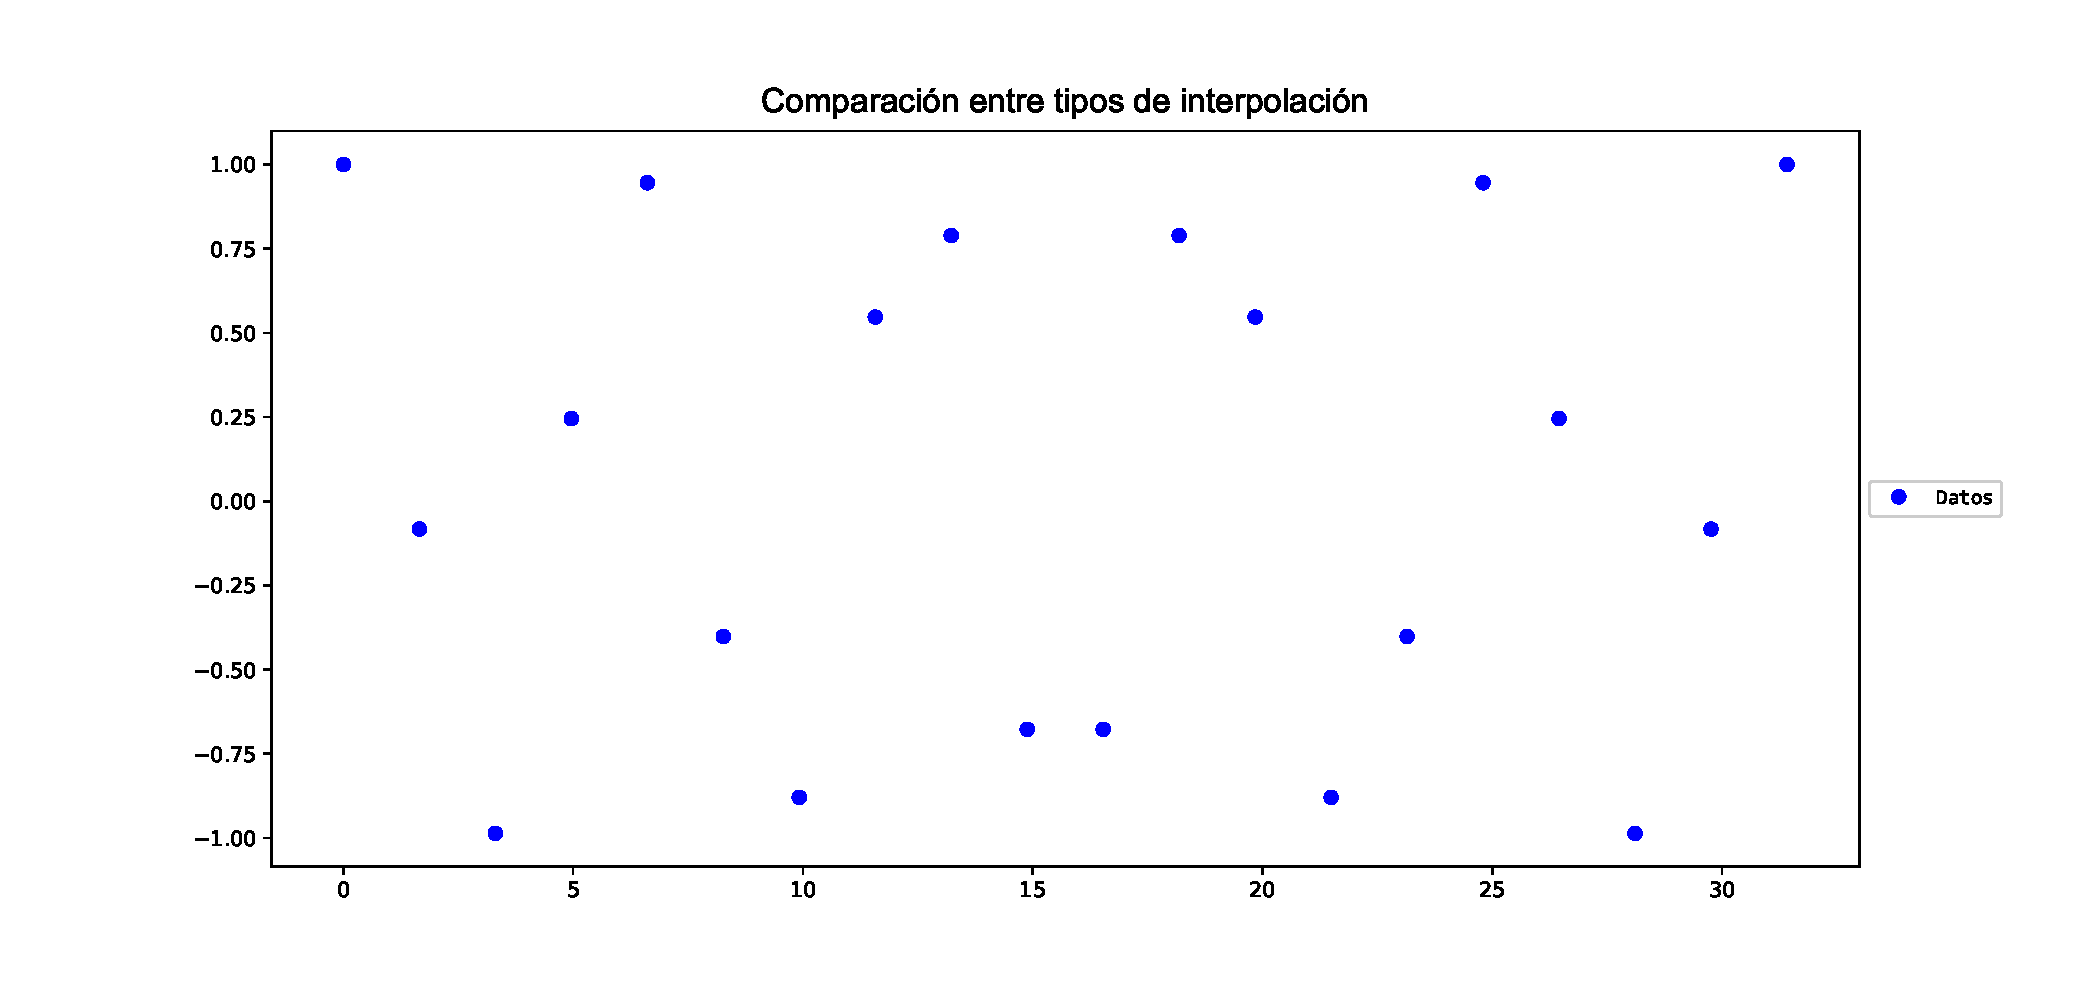
\includegraphics[scale=0.5]{Imagenes/interpolacion_01.eps}
\caption{Datos que nos servirán para interpolar.}
\end{figure}
\newpage
Ahora usaremos la función de \python\ para interpolar los datos:
\begin{lstlisting}[caption=Inteporlando con la función \funcionazul{interp1d}, basicstyle=\ttfamily\large, columns=fullflexible]
fl = interp1d(x, y, kind='linear')

fq = interp1d(x, y, kind='quadratic')

# x.min y x.max se usan para asegurar que no
# nos salimos del intervalo de interpolacion

xint = np.linspace(x.min(), x.max(), 1000)

yintl = fl(xint)

yintq = fq(xint)

plt.plot(xint, yintl, label='Lineal')
plt.plot(xint, yintq, label='Cuadratica')
plt.show()
\end{lstlisting}
En la siguiente figura vemos el resultado de la interpolación lineal:
\begin{figure}[H]
	\centering
	\hspace*{-0.2cm}\includegraphics[scale=0.5]{Imagenes/interpolacion_02.eps}
	\caption{Resultado de la interpolación lineal}
\end{figure}
Para la interpolación cuadrática, vemos en la siguiente figura el resultado:
\begin{figure}[H]
	\centering
	\hspace*{-0.2cm}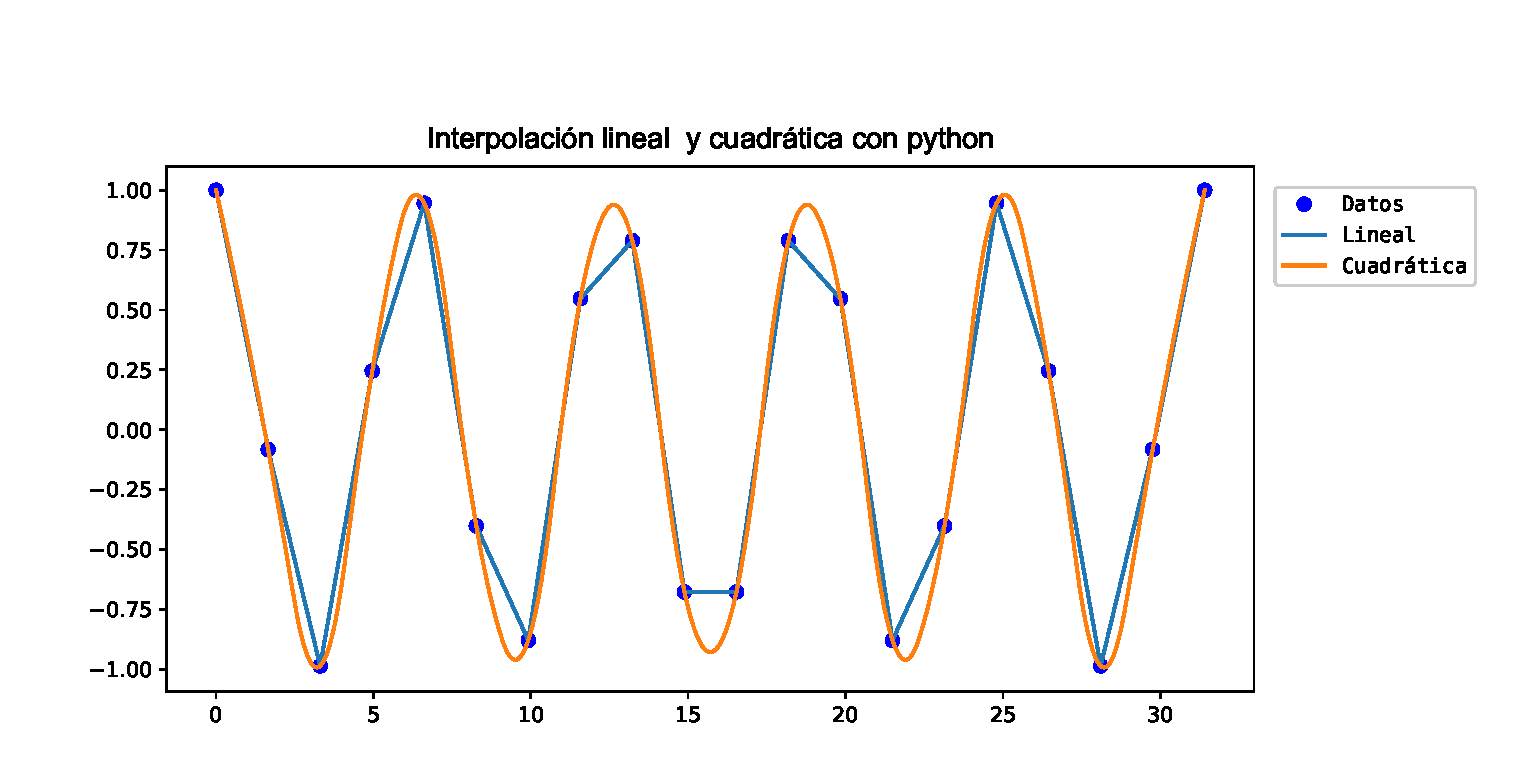
\includegraphics[scale=0.75]{Imagenes/interpolacion_03_2018.eps}
	\caption{Resultado de la interpolación usando \texttt}
\end{figure}
\subsection*{Veamos otro ejemplo.}
Utilizaremos la función \funcionazul{sinc(x)} que está contenida dentro de la librería \texttt{numpy}.
\par
La función \funcionazul{sinc (x)}, también llamada \enquote{función de muestreo}, es una función que se encuentra comúnmente de las teorías de procesamiento de señales y de las transformadas de Fourier.
\par
El nombre completo de la función es \enquote{seno cardinal}, pero es comúnmente referido por su abreviatura, \enquote{sinc}. Se define como
\[ sinc(x) = \begin{cases}
1 & \mbox{para } x = 0 \\
\dfrac{\sin x}{x} & \mbox{para cualquier otro valor} \end{cases}\]
Entonces podemos presentar el siguiente código
\begin{lstlisting}[caption=Inteporlando la función \funcionazul{sinx(x)}, basicstyle=\ttfamily\large, columns=fullflexible]
x = np.linspace(-18, 18, 36)
ruido = 0.1 * np.random.random(len(x))
senal = np.sinc(x) + ruido

interpretada = interpolate.interp1d(x, senal)
x2 = np.linspace(-18, 18, 180)
y = interpretada(x2)

cubica = interpolate.interp1d(x, senal, kind="cubic")
y2 = cubica(x2)
\end{lstlisting}
El resultado de la intepolación lo podemos ver a continuación
\begin{figure}[H]
	\centering
	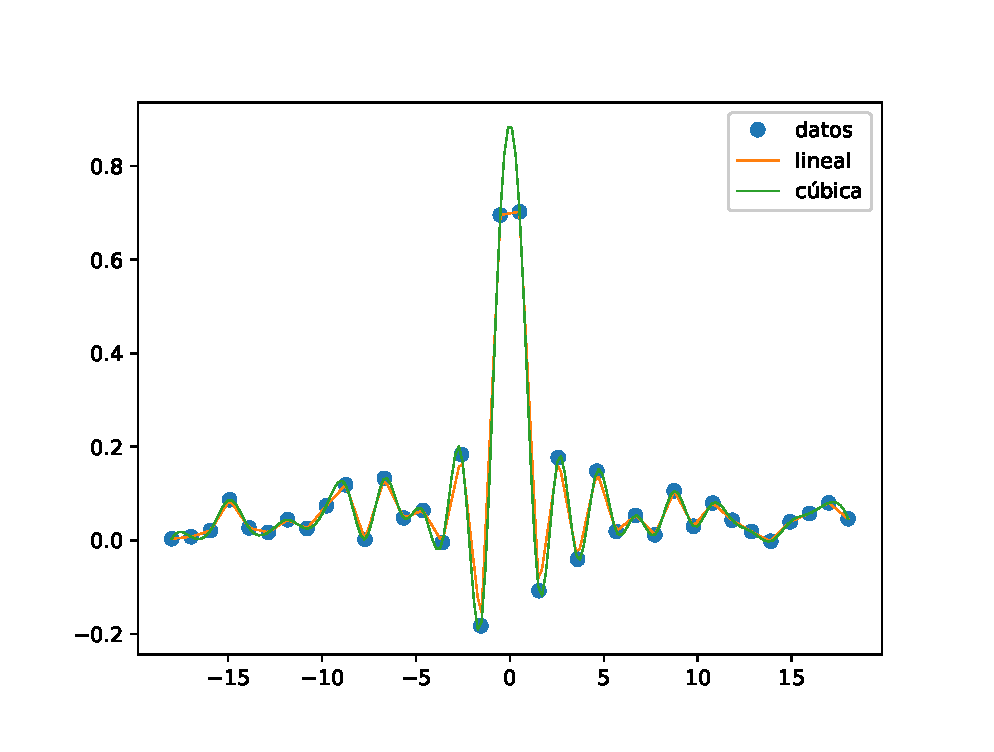
\includegraphics[scale=0.9]{Imagenes/interpolacion_04.eps}
	\caption{Interpolando puntos de la función \funcionazul{sinc(x)}}
\end{figure}
\section{Más sobre la interpolación.}
Es posible reconocer algunas características generales de la interpolación obtenida en las figuras:
\begin{enumerate}
\item Las funciones de interpolación son continuas.
\item Las funciones de interpolación pasan siempre por los puntos de datos.
\item Una función cuadrática puede dar un ajuste más malo que la interpolación lineal.
\item Aumentar el orden del polinomio no siempre conduce a un mejor ajuste.
\item Las funciones de interpolación pueden oscilar drásticamente entre los puntos de datos.
\item El ajuste empeora hacia los extremos del conjunto de datos.
\end{enumerate}
\emph{Entonces, ¿qué debo hacer al interpolar mis propios datos?}
\par
% El \enquote{spline cúbico} es el caballo de batalla en este terreno. Como se puede ver en la figura, proporciona una curva suave que parece ajustarse bien a los datos.
% \begin{figure}
% 	\centering
% 	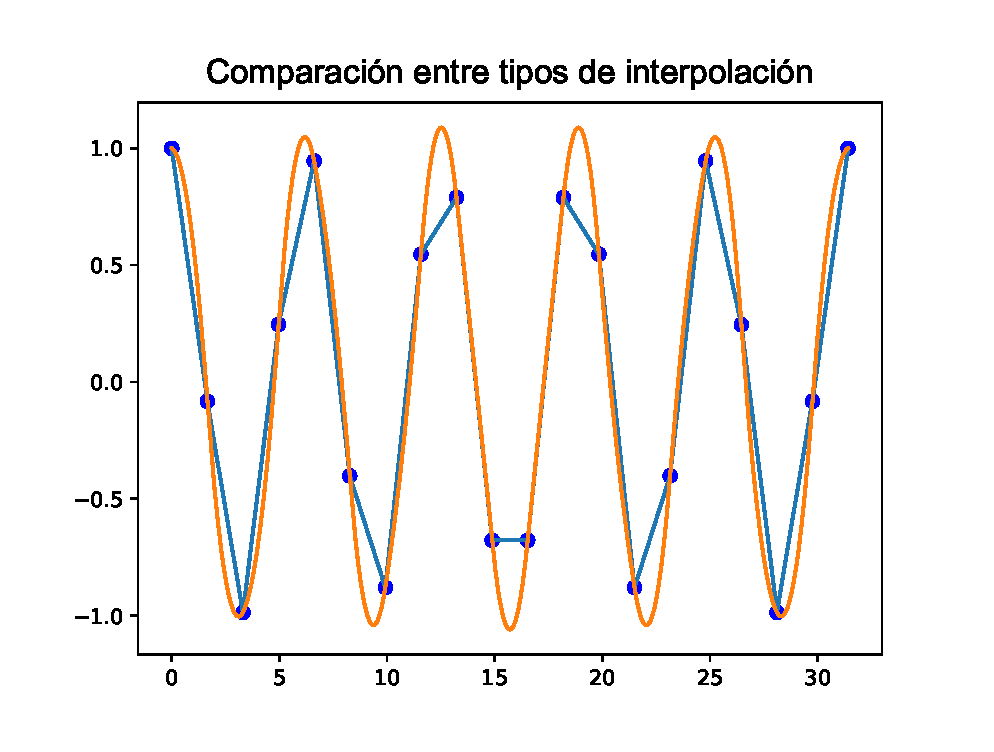
\includegraphics[scale=0.4]{Imagenes/interpolacion_03b.eps}
% 	\caption{title}
% \end{figure}
% \end{frame}
% \begin{frame}
% La suavidad se extiende más allá de lo que se ve en la gráfica: un ``spline cúbico'' tiene derivadas primera y segunda continuas.
% \\
% \bigskip
% Esta es una propiedad útil en la física, donde las derivadas primera y segunda son bastante comunes en los análisis teóricos (leyes de Newton, ecuaciones de Maxwell, ecuación de Schröedinger, etc.)
% \\
% \medskip
% \pause
% \textcolor{blue}{Una interpolación de spline cúbico es una buena opción en la mayoría de los casos}.
% \end{frame}
% \begin{frame}
% \frametitle{Precaución con las funciones de interpolación}
% Precaución: la interpolación y la extrapolación no es lo mismo.
% \\
% \bigskip
% Una buena función de interpolación puede ser una aproximación muy mala fuera del conjunto de puntos de datos utilizados. Por esta razón, las funciones generadas por \texttt{interp1d (x, y)} ni siquiera devolverán un número cuando proporcione un valor de la variable independiente fuera del rango del conjunto de datos: se obtiene un \texttt{ValueError} en su lugar.
% \end{frame}
\section{Fenómeno de Runge}
Hasta el momento hemos revisado un par de estrategias para calcular un polinomio que pase por un conjunto de datos $(x_{i}, y_{i})$, pero hay que considerar un efecto importante al respecto: no siempre el mejor polinomio será aquel el de mayor grado $n$.
\par
Veamos el siguiente ejemplo: sea la función:
\[ f(x) = \dfrac{1}{1 + 25 x^{2}}\]
La gráfica de la función $f(x)$ es la siguiente
\begin{figure}[H]
	\centering
	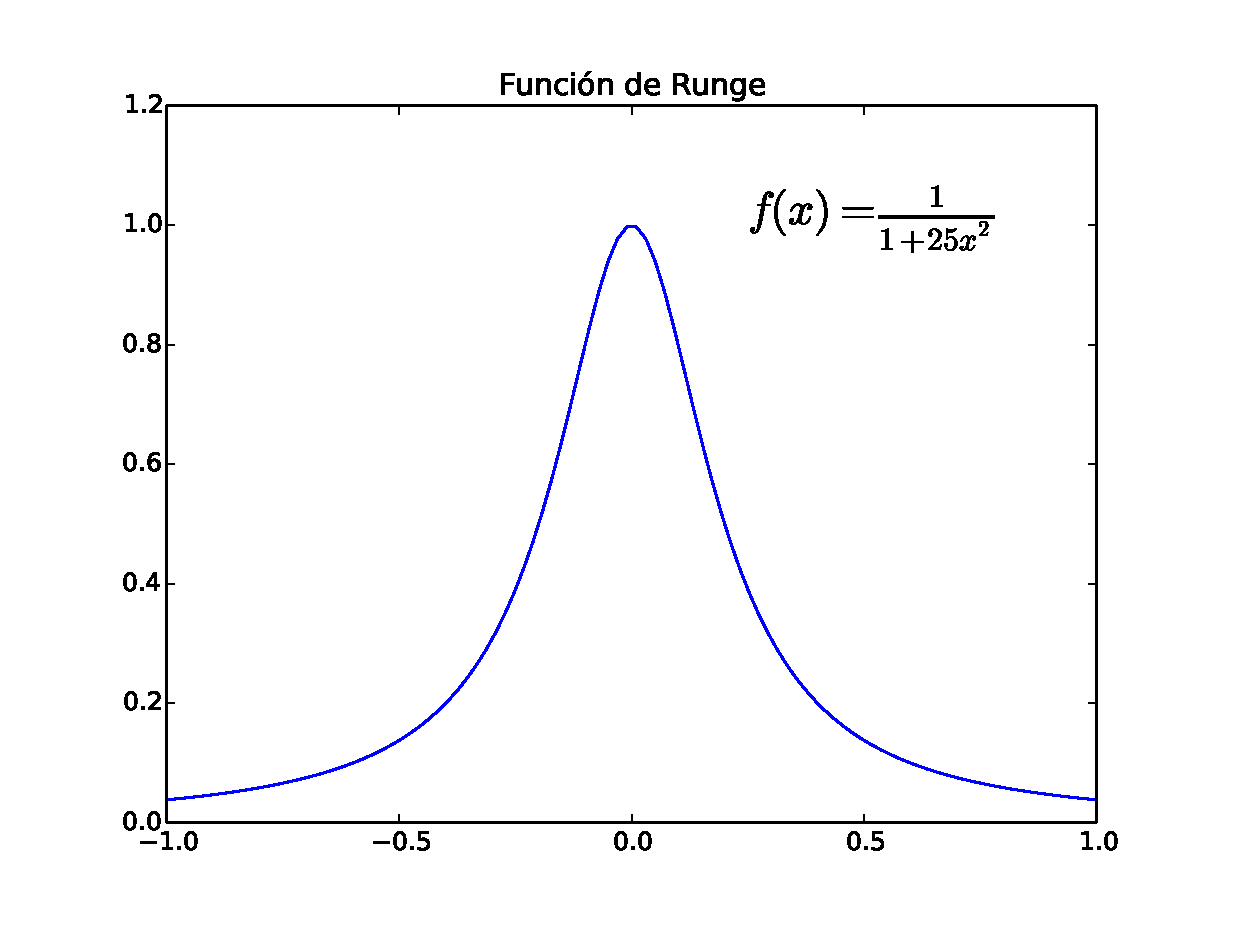
\includegraphics[scale=0.8]{Imagenes/Funcion_Runge_01.eps}
	\caption{Función de Runge}
\end{figure}
\subsection*{Elección de puntos para interpolar.}
Hagamos una elección aleatoria de puntos:
\begin{figure}[H]
	\centering
	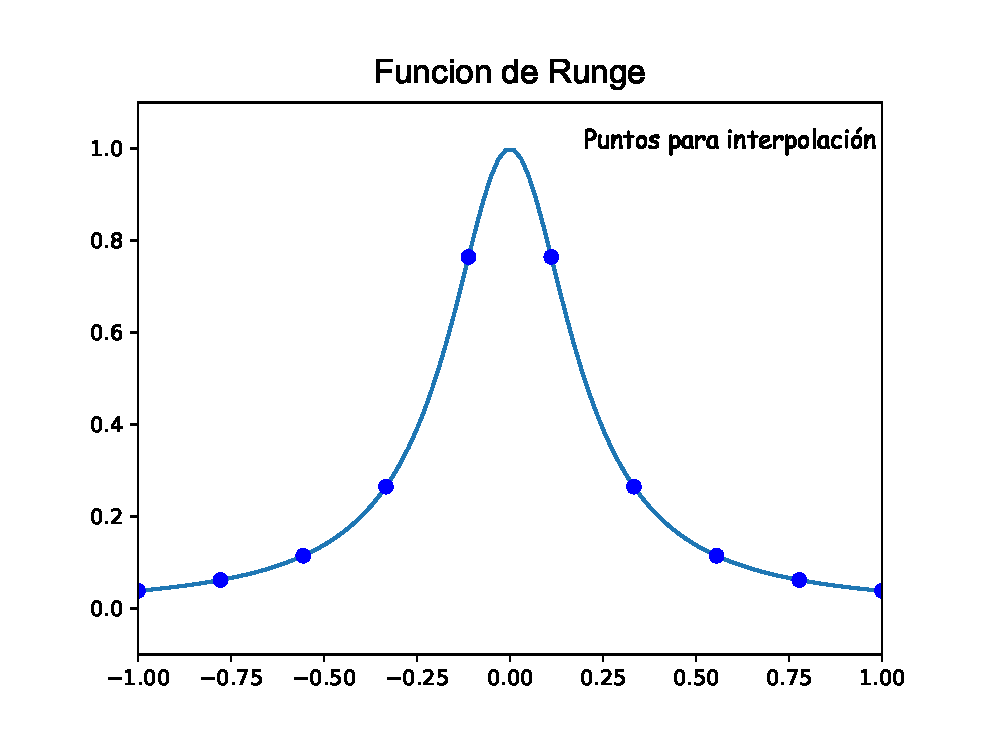
\includegraphics[scale=0.8]{Imagenes/Funcion_Runge_2017_01.eps}
	\caption{Elección de puntos.}
\end{figure}
Si hacemos una interpolación mediante el método de Lagrange, obtendremos lo siguiente:
\begin{figure}[H]
	\centering
	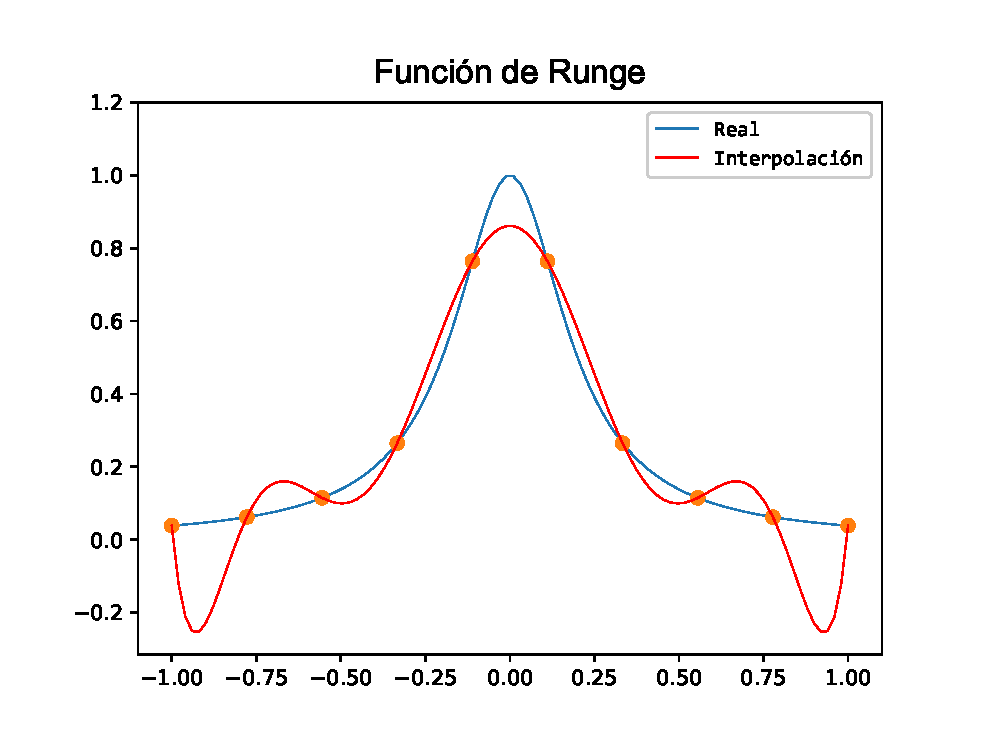
\includegraphics[scale=0.8]{Imagenes/Funcion_Runge_2017_02.eps}
	\caption{Gráfica de la interpolación con Lagrange.}
\end{figure}
\emph{¿Qué hacemos al respecto?}
\par
Como hemos visto en la gráfica anterior, la función que resulta del proceso de interpolación \enquote{oscila} a través de los puntos que deseamos interpolar; aquí el caso es que si aumentamos el grado del polinomio, los resultados serán aún más indeseables.
\par
La pregunta obligada es: \textcolor{blue}{¿qué podemos hacer para mejorar la interpolación?}
\subsection{¿Qué es un spline?}
En términos nada riguroso, se puede decir que un spline es una función definida por una familia de polinomios \enquote{sociables}, donde el término sociable se usa para indicar que los polinomios que constituyen una función \emph{spline}, están estrechamente vinculados.
\par
El nombre de \emph{spline}, viene del inglés ya que es un instrumento que utilizaban los ingenieros navales para dibujar curvas suaves, forzadas a pasar por un conjunto de puntos prefijados.
\subsection{Las tres B's de los splines}
El uso de las funciones splines tiene mucha aceptación y popularidad se deben a tres razones básicas, ya que son:
\begin{enumerate}
\item \textbf{Buenos:} Se  pueden usar en la solución de una gran variedad de problemas.
\item \textbf{Bonitos:} La teoría matemática en que se basan es muy simple y a la vez elegante.
\item \textbf{Baratos:} Ya que su cálculo es muy sencillo y económico.
\end{enumerate}
\section{Manejando splines con \python}
Usaremos la librería \funcionazul{scipy} que contiene varias funciones con las que ahorramos tiempo para manejar splines y ajustar funciones sociables a un conjunto de datos.
\par
 No está de más que revises la teoría al respecto, en la mayoría de los libros de análisis numérico, podrás encontrar la construcción matemática y formal de los splines.
\subsection*{Funciones para los splines}
Necesitaremos de dos pasos para el uso de splines con \python, de la librería: \\
\funcionazul{scipy.interpolate}, las cuales son:
\begin{enumerate}
\item \funcionazul{splrep}: Calcula el spline básico (B-spline) para una curva 1-D.
\\
\medskip
Dado un conjunto de puntos $(x[i],y[i])$, la función determina una aproximación con un spline suave de grado $k$ en el intervalo $xb \leq x \leq xe$.
\item \funcionazul{splev}: Evalúa un B-spline o sus derivadas.
\\
\medskip
Dados los nodos y coeficientes de un B-spline, calcula el valor del polinomio suave y sus derivadas.
\end{enumerate}
La sintaxis mínima de la función \funcionazul{splrep} es la siguiente:
\\
\texttt{splrep(x, y, xb=None, xe=None, k=3)}
donde:
\begin{itemize}
\item $x$, $y$ : son arreglos de valores que definen la función $y = f(x)$.
\item $xb$, $xe$ : es el intervalo en donde se realizará el ajuste. En caso de que no se proporcione, se tomarán por defecto $x[0]$ y $x[-1]$, respectivamente.
\item $k$ : es un entero (\texttt{int}), es un argumento opcional. Corresponde al grado del spline. Se recomienda usar splines cúbicos.
\end{itemize}
La sintaxis mínima para la función \funcionazul{splev} es:
\\
\texttt{splev(x, tck)}
donde
\begin{itemize}
\item $x$ : es un arreglo. Considera los nodos y los coeficientes del B-spline, calcula el valor del polinomio suavizado.
\item $tck$ : es un tupla de 3 elementos. Representa la secuencia de elementos que devuelve \funcionazul{splrep} que contiene los nodos, los coeficientes y el grado del spline.
\end{itemize}
Hagamos un ejemplo para revisar el uso de los splines, seguiremos con la función de Runge:
\begin{lstlisting}[caption=Código para usar un spline, style=FormattedNumber, basicstyle=\linespread{1.1}\ttfamily=\small, columns=fullflexible]
import matplotlib.pyplot as plt
import scipy.interpolate as si
import numpy as np

x = np.linspace(-1, 1, 100)
y = 1./(1 + 25 * x**2)

def trazadorCub(n):
    xi = np.linspace(-1, 1, n)
    yi = 1./(1 + 25 * xi**2)
    tck = si.splrep(xi, yi)
    return tck

tck = trazadorCub(8)
ys_8_ = si.splev(x, tck)

tck = trazadorCub(12)
ys_12_ = si.splev(x, tck)

plt.plot(x, y)
plt.plot(x, ys_8_, '+g-', label='n=8')
plt.plot(x, ys_12_, '+r-', label ='n=12')
plt.legend(loc='best')
plt.title('Interpolacion con splines cubicos')
plt.ylim(-0.2, 1.2)
plt.show()
\end{lstlisting}
La función \funcionazul{trazadorCub(n)}, genera el número de puntos \enquote{medidos o experimentales}, en el primer caso, genera $8$ puntos espaciados de manera equidistante, mientras que en el segundo caso, tenemos $12$ puntos distribuidos sobre el eje$x$.
\par
Al usar la función \funcionazul{splev}, se introducen $100$ valores para generar el spline cúbico. La gráfica que se genera y en donde podemos ver el resultado al calcular el spline, es la siguiente:
\begin{figure}[H]
	\centering
	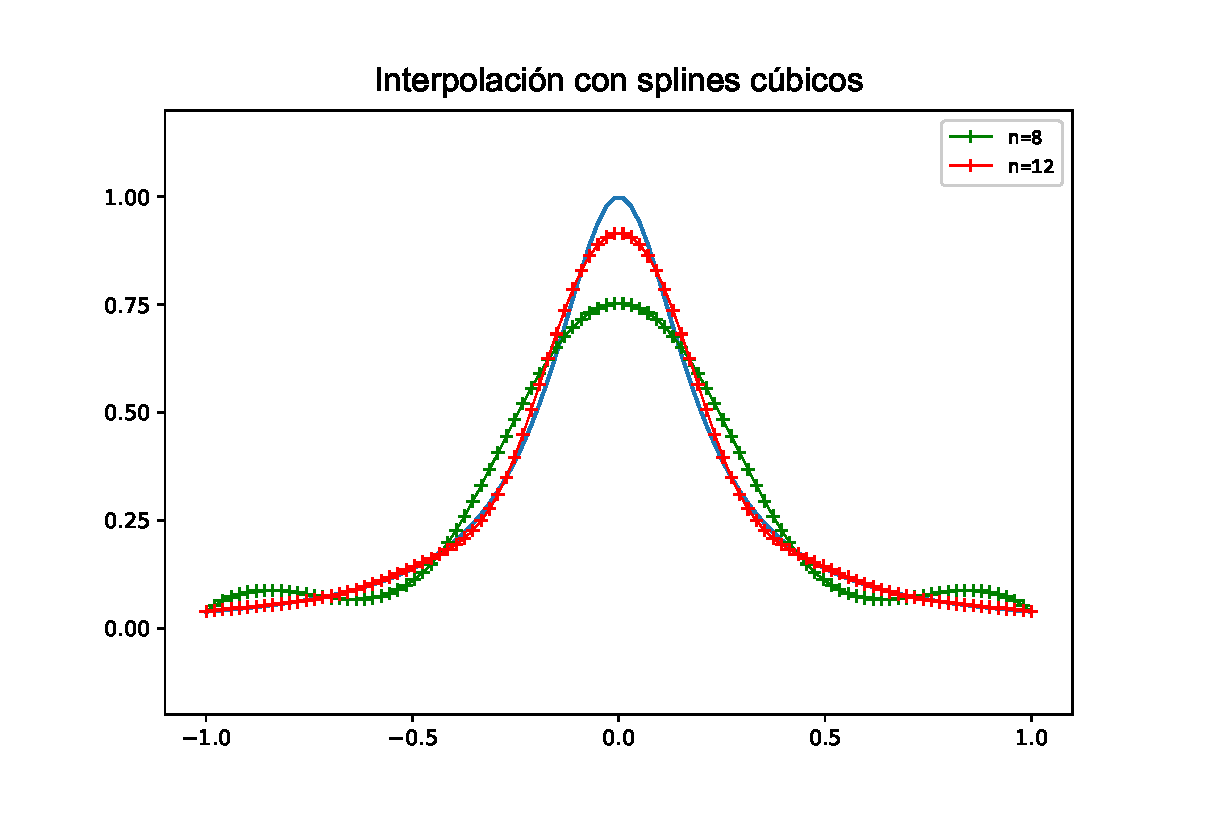
\includegraphics[scale=0.8]{Imagenes/Funcion_Runge_2017_03.eps}
	\caption{Uso de los splines en \python.}
\end{figure}
\end{document}